\setauthor{\secondauthor}

Nutzer:innen können Mitschriften hochladen und einem Fach sowie einem 
Themenpool zuordnen. Beim Upload müssen ein Titel, eine Beschreibung 
sowie die zuständige Lehrkraft für die Freigabe angegeben werden. 
Die Mitschrift wird dabei automatisch dem gewählten Fach und Themenpool 
zugeordnet, was die spätere Navigation für alle Nutzer:innen erleichtert.

\begin{figure}[H]
    \centering
    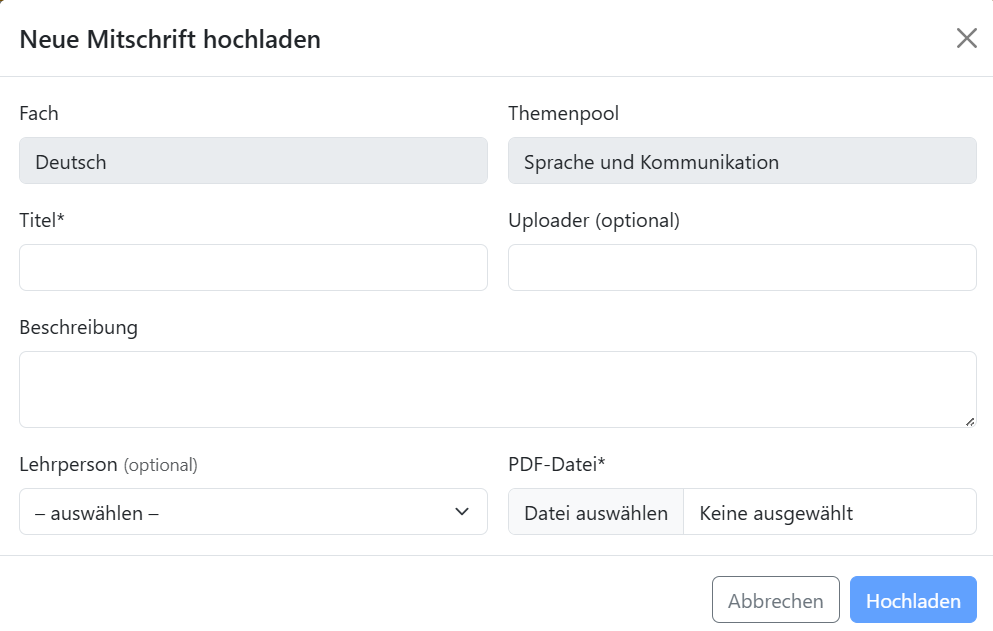
\includegraphics[width=0.7\textwidth]{pics/ab5.png}
    \caption{Mitschriften-Upload-Formular}
    \label{fig:mitschriften-upload}
\end{figure}

\paragraph{Upload als Schüler:in}

Schüler:innen können eigene Mitschriften hochladen. Solange die 
Mitschrift noch nicht freigegeben ist, wird sie mit dem Status 
\textit{PENDING} dargestellt und ist nur für die jeweilige Schüler:in 
sichtbar. Solange eine Mitschrift noch den Status \textit{PENDING} hat, 
kann sie von der Schüler:in noch bearbeitet oder gelöscht werden. 
Nach der Freigabe durch eine Lehrkraft erhält sie den Status 
\textit{APPROVED} und ist für alle Nutzer:innen sichtbar.

Abbildung~\ref{fig:mitschriften} zeigt die Mitschriftenübersicht mit 
dem Status der einzelnen Mitschriften.

\begin{figure}[H]
    \centering
    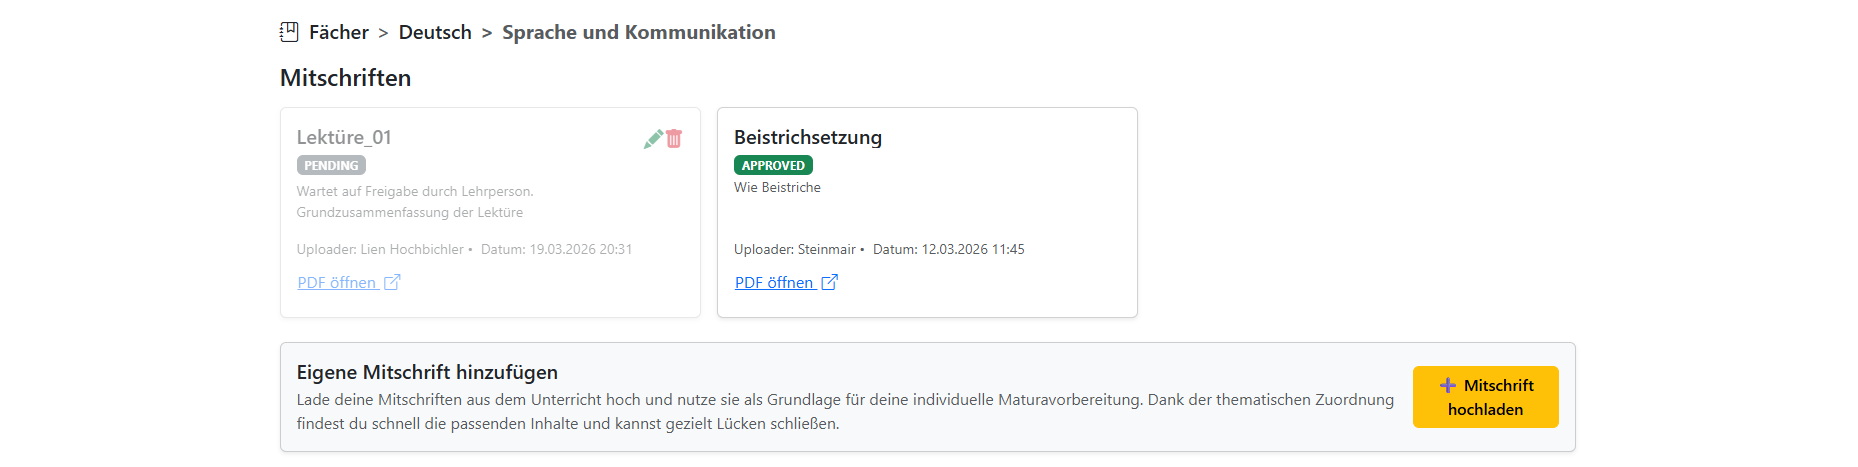
\includegraphics[width=0.9\textwidth]{pics/ab4.png}
    \caption{Mitschriftenübersicht}
    \label{fig:mitschriften}
\end{figure}

\paragraph{Upload als Lehrkraft}

Lehrkräfte können Mitschriften hochladen, die sofort öffentlich sichtbar 
sind, ohne einen Freigabeprozess durchlaufen zu müssen. Zusätzlich können 
sie alle Mitschriften der Plattform, unabhängig vom Ersteller, bearbeiten 
oder löschen.